% !TEX root =  ../supplementary.tex
\section{A Joint Model for the Longitudinal PSA, and Time to Gleason $\geq$ 7}
\label{sec:jm_framework}

\subsection{Study Cohort}
Prostate Cancer International Active Surveillance (PRIAS) is an ongoing prospective cohort study of men with low- and very-low risk PCa diagnoses \citep{bul2013active}. More than 100 medical centers from 17 countries contribute in PRIAS, using a common study protocol (\url{www.prias-project.org}). We used the data collected between December~2006 (beginning of PRIAS study) and May~2019. The PSA was measured every three months until year two of follow-up and every six months thereafter. Biopsy schedule was year one, four, seven, and ten, and additional yearly biopsies when PSA doubling time is between zero and ten years. The primary event of this work is Gleason~$\geq$~7 (GS7). It was observed in 1134 patients, but 2250 were provided treatment (see Table \ref{table:prias_summary}). Treatment in absence of GS7 may have been advised on the basis of PSA, number of biopsy cores with cancer, anxiety, or other reasons. We focused only on GS7 because of its strong association with cancer-related outcomes. Due to the periodical nature of biopsies, the time of GS7 was only known as a time interval in which it occurred.

\begin{table}[!htb]
\small\sf\centering
\caption{\textbf{Patient characteristics for the PRIAS dataset}. The primary event of interest is Gleason~$\geq$~7. IQR: interquartile range, PSA: prostate-specific antigen.}
\label{table:prias_summary}
\begin{tabular}{lr}
\hline
\hline
Characteristic & Value\\
\hline
Total patients & 7813\\
Gleason~$\geq$~7 (primary event) & 1134\\
Treatment & 2250\\
Watchful waiting & 334\\
Loss to follow-up & 250\\
Death (unrelated to prostate cancer) & 95\\
Death (related to prostate cancer) & 2\\
\hline
Median age at diagnosis (years) & 66 (IQR: 61--71)\\
Median follow-up period per patient (years) &  1.8 (IQR: 0.9--4.0)\\
Total PSA measurements & 67578\\
Median number of PSA measurements per patient &  6 (IQR: 4--12)\\
Median PSA value (ng/mL) & 5.7 (IQR: 4.1--7.7)\\
Total biopsies & 15686\\
Median number of biopsies per patient &  2 (IQR: 1--2)\\
\hline
\end{tabular}
\end{table}

\subsection{Model Definition}
\label{subsec:model_def}
Let $T_i^*$ denote the true time of GS7 for the ${i\mbox{-th}}$ patient included in PRIAS. Since biopsies are conducted periodically, $T_i^*$ is observed with interval censoring ${l_i < T_i^* \leq r_i}$. When GS7 is observed for the patient at his latest biopsy time $r_i$, then $l_i$ denotes the time of the second latest biopsy. Otherwise, $l_i$ denotes the time of the latest biopsy and ${r_i=\infty}$. Let $\boldsymbol{y}_{i}$ denote his observed PSA longitudinal measurements. The observed data of all $n$ patients is denoted by ${\mathcal{D}_n = \{l_i, r_i, \boldsymbol{y}_{i}; i = 1, \ldots, n\}}$.

\begin{figure}
\centerline{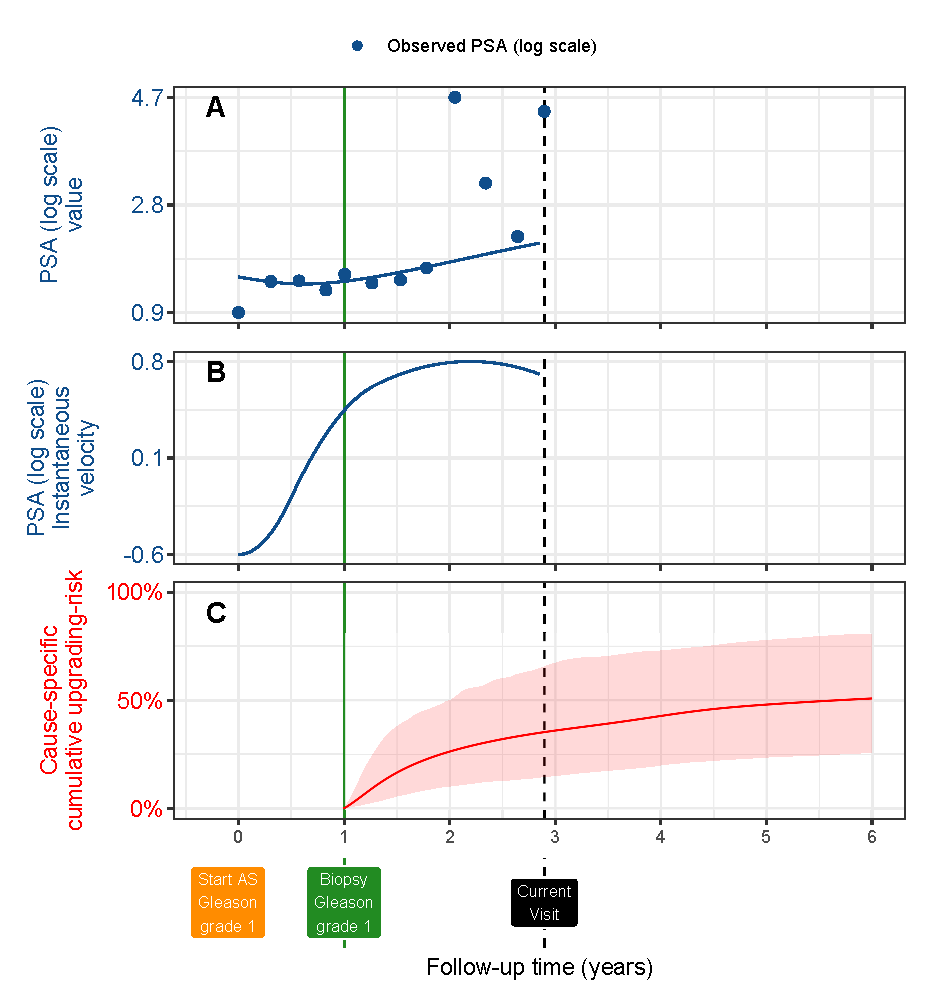
\includegraphics[width=\columnwidth]{images/jmExplanationPlot_113.eps}}
\caption{\textbf{Illustration of the joint model fitted to the PRIAS dataset}. \textbf{Panel~A:} shows the observed and fitted $\log_2(\mbox{PSA} + 1)$ measurements (Equation~\ref{eq:long_model_psa}). \textbf{Panel~B:} shows the estimated $\log_2(\mbox{PSA} + 1)$ velocity over time, mathematically derived from Equation~(\ref{eq:long_model_psa}). The cumulative risk of Gleason $\geq$ 7 (Equation~\ref{eq:rel_risk_model}) shown in \textbf{Panel~C}, depends on the fitted $\log_2(\mbox{PSA} + 1)$ value and velocity, and the time of the latest biopsy (year 1 in this case).}
\label{fig:jmExplanationPlot_113}
\end{figure}

In our joint model, the patient-specific PSA measurements over time are modeled using a linear mixed effects sub-model. It is given by (see Panel~A, Figure~\ref{fig:jmExplanationPlot_113}):
\begin{equation}
\label{eq:long_model_psa}
\begin{split}
    \log_2 \big\{y_{i}(t) + 1\big\} &= m_{i}(t) + \varepsilon_{i}(t),\\
    m_{i}(t) &= \beta_{0} + b_{0i} + \sum_{k=1}^4 (\beta_{k} + b_{ki})  B_k\Big(\frac{t-2}{2},\frac{\mathcal{K}-2}{2}\Big) + \beta_{5} \mbox{age}_i,
    \end{split}
\end{equation}
where, $m_{i}(t)$ denotes the measurement error free value of $\log_2 (\mbox{PSA} + 1)$ transformed \citep{pearson1994mixed,lin2000latent} measurements at time $t$. We model it non-linearly over time using B-splines \citep{de1978practical}. To this end, our B-spline basis function $B_k\{(t-2)/2,(\mathcal{K}-2)/2\}$ has 3 internal knots at $\mathcal{K} = \{0.5, 1.3, 3\}$ years, which are the three quartiles of the observed follow-up times. The boundary knots of the spline are at 0 and 6.3 years (95-th percentile of the observed follow-up times). We mean centered (mean 2 years) and standardized (standard deviation 2 years) the follow-up time $t$ and the knots of the B-spline $\mathcal{K}$ during parameter estimation for better convergence. The fixed effect parameters are denoted by ${\{\beta_{0},\ldots,\beta_{5}\}}$, and ${\{b_{0i}, \ldots, b_{4i}\}}$ are the patient specific random effects. The random effects follow a multivariate normal distribution with mean zero and variance-covariance matrix $\boldsymbol{D}$. The error $\varepsilon_{i}(t)$ is assumed to be t-distributed with three degrees of freedom (see Appendix~B.1) and scale $\sigma$, and is independent of the random effects. 

To model the impact of PSA measurements on the risk of GS7, our joint model uses a relative risk sub-model. More specifically, the hazard of GS7 denoted as $h_i(t)$, and the cumulative risk of GS7 denoted as $R_i(t)$, at a time $t$ are (see Panel~C, Figure~\ref{fig:jmExplanationPlot_113}):
\begin{equation}
\label{eq:rel_risk_model}
\begin{split}
    h_i(t) &= h_0(t) \exp\Big(\gamma \mbox{age}_i +\alpha_{1} m_{i}(t) + \alpha_{2} \frac{\partial m_{i}(t)}{\partial {t}}\Big),\\
    R_i(t) &= \exp\Big\{-\int_0^{t} h_i(s)\mathrm{d}{s}\Big\},
    \end{split}
\end{equation}
where, $\gamma$ is the parameter for the effect of age. The impact of PSA on the hazard of GS7 is modeled in two ways, namely the impact of the error free underlying PSA value $m_{i}(t)$ (see Panel~A, Figure~\ref{fig:jmExplanationPlot_113}), and the impact of the underlying PSA velocity $\partial m_{i}(t)/\partial {t}$ (see Panel~B, Figure~\ref{fig:jmExplanationPlot_113}). The corresponding parameters are $\alpha_{1}$ and $\alpha_{2}$, respectively. Lastly, $h_0(t)$ is the baseline hazard at time t, and is modeled flexibly using P-splines \citep{eilers1996flexible}. More specifically:
\begin{equation*}
\log{h_0(t)} = \gamma_{h_0,0} + \sum_{q=1}^Q \gamma_{h_0,q} B_q(t, \boldsymbol{v}),
\end{equation*}
where $B_q(t, \boldsymbol{v})$ denotes the $q$-th basis function of a B-spline with knots $\boldsymbol{v} = v_1, \ldots, v_Q$ and vector of spline coefficients $\gamma_{h_0}$. To avoid choosing the number and position of knots in the spline, a relatively high number of knots (e.g., 15 to 20) are chosen and the corresponding B-spline regression coefficients $\gamma_{h_0}$ are penalized using a differences penalty \citep{eilers1996flexible}.

%\subsection{Issue of PSA Dependent Interval Censored Time of GS7 in PRIAS}
%\label{subsec:ascertainment_bias}
%The true time $T^*_i$ of GS7 is not known for any of the patients in PRIAS. In order to detect GS7, PRIAS uses a fixed schedule of biopsies wherein biopsies are conducted at year one, year four, year seven and year ten of follow-up, and every five years thereafter. However, PRIAS switches to a more frequent annual biopsy schedule for faster-progressing patients. These are patients with PSA doubling time (PSA-DT) between zero and ten years, which is measured as the inverse of the slope of the regression line through the base two logarithm of PSA values. Thus, the interval $l_i < T_i^* \leq r_i$ in which GS7 is detected depends on the observed PSA values. 

%Given the issue of PSA dependent interval censoring it is natural to question in this scenario if the parameters of the joint model are affected by these two. However, because the parameters of the joint model are estimated using a full likelihood approach \citep{tsiatis2004joint}, the joint model allows the schedule of biopsies, as well as censoring to depend upon the observed PSA measurements (e.g., via PSA-DT), under the condition that the model is correctly specified. To show this, consider the following full general specification of the joint model that we use. Let $\boldsymbol{y}_{i}$ denote the observed DRE and PSA measurements for the $i$-th patient, and $l_i, r_i$ denote the two time points of the interval in which GR occurs for the $i$-th patient. In addition let $T_i^S$ and $\mathcal{V}_{i}$ denote the schedule of biopsies, and the schedule of DRE and PSA measurements, respectively. Let $G^*_i$ denote the time of removal from AS without observing GS7. Under the assumption that $T_i^S, G^*_i, \mathcal{V}_{i}$ may depend upon only the observed data $\boldsymbol{y}_{i}$, the joint likelihood of the various processes is given by:
%\begin{align*}
%p( l_i, r_i, T_i^S, G^*_i, \boldsymbol{y}_{i}, \mathcal{V}_{i} \mid \boldsymbol{\theta}, \boldsymbol{\psi}) &= p(\boldsymbol{y}_{i}, l_i, r_i \mid \boldsymbol{\theta}) \times p(T_i^S, G^*_i, \mathcal{V}_{i} \mid \boldsymbol{y}_{i}, \boldsymbol{\psi}).
%\end{align*}
%From this decomposition we can see that even if the processes $T_i^S, G^*_i, \mathcal{V}_{i}$ may be determined from $\boldsymbol{y}_{i}$, if we are interested in the parameters $\boldsymbol{\theta}$ of the joint distribution of longitudinal and event outcomes, we can maximize the likelihood based on the first term and ignore the second term. In other words, the second term will not carry information for $\boldsymbol{\theta}$. Lastly, since we use a full likelihood approach with an interval censoring specification, the estimates that we obtain are consistent and asymptotically unbiased \citep{gentleman1994maximum}, despite the interval censoring observed. 

\subsection{Parameter Estimation}
We estimate the parameters of the joint model using Markov chain Monte Carlo (MCMC) methods under the Bayesian framework. Let $\boldsymbol{\theta}$ denote the vector of all of the parameters of the joint model. The joint model postulates that given the random effects, the time of GS7, and the PSA measurements taken over time are all mutually independent. Under this assumption the posterior distribution of the parameters is given by:
\begin{align*}
p(\boldsymbol{\theta}, \boldsymbol{b} \mid \mathcal{D}_n) & \propto \prod_{i=1}^n p(l_i, r_i, \boldsymbol{y}_{i}, \mid \boldsymbol{b}_i, \boldsymbol{\theta}) p(\boldsymbol{b}_i \mid \boldsymbol{\theta}) p(\boldsymbol{\theta})\\
& \propto \prod_{i=1}^n p(l_i, r_i \mid \boldsymbol{b}_i, \boldsymbol{\theta}) p(\boldsymbol{y}_{i} \mid \boldsymbol{b}_i, \boldsymbol{\theta}) p(\boldsymbol{b}_i \mid \boldsymbol{\theta}) p(\boldsymbol{\theta}),\\
p(\boldsymbol{b}_i \mid \boldsymbol{\theta}) &= \frac{1}{\sqrt{(2 \pi)^q \text{det}(\boldsymbol{D})}} \exp(\boldsymbol{b}_i^T \boldsymbol{D}^{-1} \boldsymbol{b}_i),
\end{align*}
where, the likelihood contribution of the PSA outcome, conditional on the random effects is:
\begin{equation*}
p(\boldsymbol{y}_{i} \mid \boldsymbol{b}_i, \boldsymbol{\theta}) = \frac{1}{\big(\sqrt{2 \pi \sigma^2}\big)^{n_{i}}} \exp\bigg(-\frac{{\lVert{\boldsymbol{y}_{i} - \boldsymbol{m}_{i}}\rVert}^2}{\sigma^2}\bigg),
\end{equation*}
The likelihood contribution of the time of GS7 outcome is given by:
\begin{equation}
\label{web_eq : likelihood_contribution_survival}
p(l_i,r_i\mid \boldsymbol{b}_i,\boldsymbol{\theta}) = \exp\Big\{-\int_0^{l_i} h_i(s)\mathrm{d}{s}\Big\} - \exp\Big\{-\int_0^{r_i}h_i(s)\mathrm{d}{s}\Big\}.
\end{equation}
The integral in (\ref{web_eq : likelihood_contribution_survival}) does not have a closed-form solution, and therefore we use a 15-point Gauss-Kronrod quadrature rule to approximate it.

We use independent normal priors with zero mean and variance 100 for the fixed effects $\{\beta_{0},\ldots,\beta_{5}\}$, and inverse Gamma prior with shape and rate both equal to 0.01 for the parameter $\sigma^2$. For the variance-covariance matrix $\boldsymbol{D}$ of the random effects we take inverse Wishart prior with an identity scale matrix and degrees of freedom equal to 5 (number of random effects). For the relative risk model's parameter $\gamma$ and the association parameters $\alpha_{1}, \alpha_{2}$, we use independent normal priors with zero mean and variance 100.

\subsection{Parameter Estimates}
The joint model was fitted using the R package \textbf{JMbayes} \citep{rizopoulosJMbayes}. This package utilizes the Bayesian methodology to estimate model parameters. The corresponding posterior parameter estimates are shown in Table~\ref{tab:PSA_long} (longitudinal sub-model for PSA outcome) and Table~\ref{tab:PSA_survival} (relative risk sub-model). The parameter estimates for the variance-covariance matrix $\boldsymbol{D}$ from the longitudinal sub-model for PSA are shown in the following Table~\ref{tab:D_matrix}:
\begin{table}[!htb]
\small\sf\centering
\caption{Estimated variance-covariance matrix $\boldsymbol{D}$ of the random effects ${\boldsymbol{b}=(b_{0}, b_{1}, b_{2}, b_{3}, b_{4})}$ (see \ref{subsec:model_def}) from the joint model fitted to the PRIAS dataset. The variances of the random effects are highlighted along the diagonal of the variance-covariance matrix.}
\label{tab:D_matrix}
\begin{tabular}{lrrrrr}
\hline
Random Effects    & $b_{0}$    & $b_{1}$   & $b_{2}$   & $b_{3}$   & $b_{4}$    \\
\hline
$b_{0}$ & \textbf{0.229} & 0.030 & 0.023 & 0.073 & 0.007 \\
$b_{1}$ & 0.030 & \textbf{0.149} & 0.098 & 0.171 & 0.085 \\
$b_{2}$ & 0.023 & 0.098 & \textbf{0.276} & 0.335 & 0.236 \\
$b_{3}$ & 0.073 & 0.171 & 0.335 & \textbf{0.560} & 0.359 \\
$b_{4}$ & 0.007 & 0.085 & 0.236 & 0.359 & \textbf{0.351} \\
\hline
\end{tabular}
\end{table}

For the PSA mixed effects sub-model parameter estimates (see Equation \ref{eq:long_model_psa}), in Table~\ref{tab:PSA_long} we can see that the age of the patient trivially affects the baseline ${\log_2(\mbox{PSA} + 1)}$ measurement. Since the longitudinal evolution of ${\log_2 (\mbox{PSA} + 1)}$ measurements is modeled with non-linear terms, the interpretation of the coefficients corresponding to time is not straightforward. In lieu of the interpretation, in Figure~\ref{fig:fitted_9subject_psa} we present plots of observed versus fitted PSA profiles for nine randomly selected patients. 
\begin{table}[!htb]
\small\sf\centering
\caption{Estimated mean and 95\% credible interval for the parameters of the longitudinal sub-model (see Equation \ref{eq:long_model_psa}) for the PSA outcome.}
\label{tab:PSA_long}
\begin{tabular}{lrrrrr}
\hline
Variable                         & Mean & Std. Dev & 2.5\%  & 97.5\% & P     \\
\hline
Intercept & 2.129    & 0.060  & 2.009 & 2.244 & \textless0.001 \\
Age & 0.008    & 0.001 & 0.007 & 0.010   &\textless0.001 \\
Spline: [0.0, 0.5] years & 0.063    & 0.007 & 0.051 & 0.075  & \textless0.001 \\
Spline: [0.5, 1.3] years & 0.196    & 0.010  & 0.177 & 0.217  & \textless0.001 \\
Spline: [1.3, 3.0] years & 0.244    & 0.014 & 0.217 & 0.272  & \textless0.001 \\
Spline: [3.0, 6.3] years & 0.382    & 0.014 & 0.356 & 0.410 &  \textless0.001 \\
$\sigma$ & 0.139    & 0.001 & 0.138 & 0.140  & \\
\hline
\end{tabular}
\end{table}

\begin{figure}
\centerline{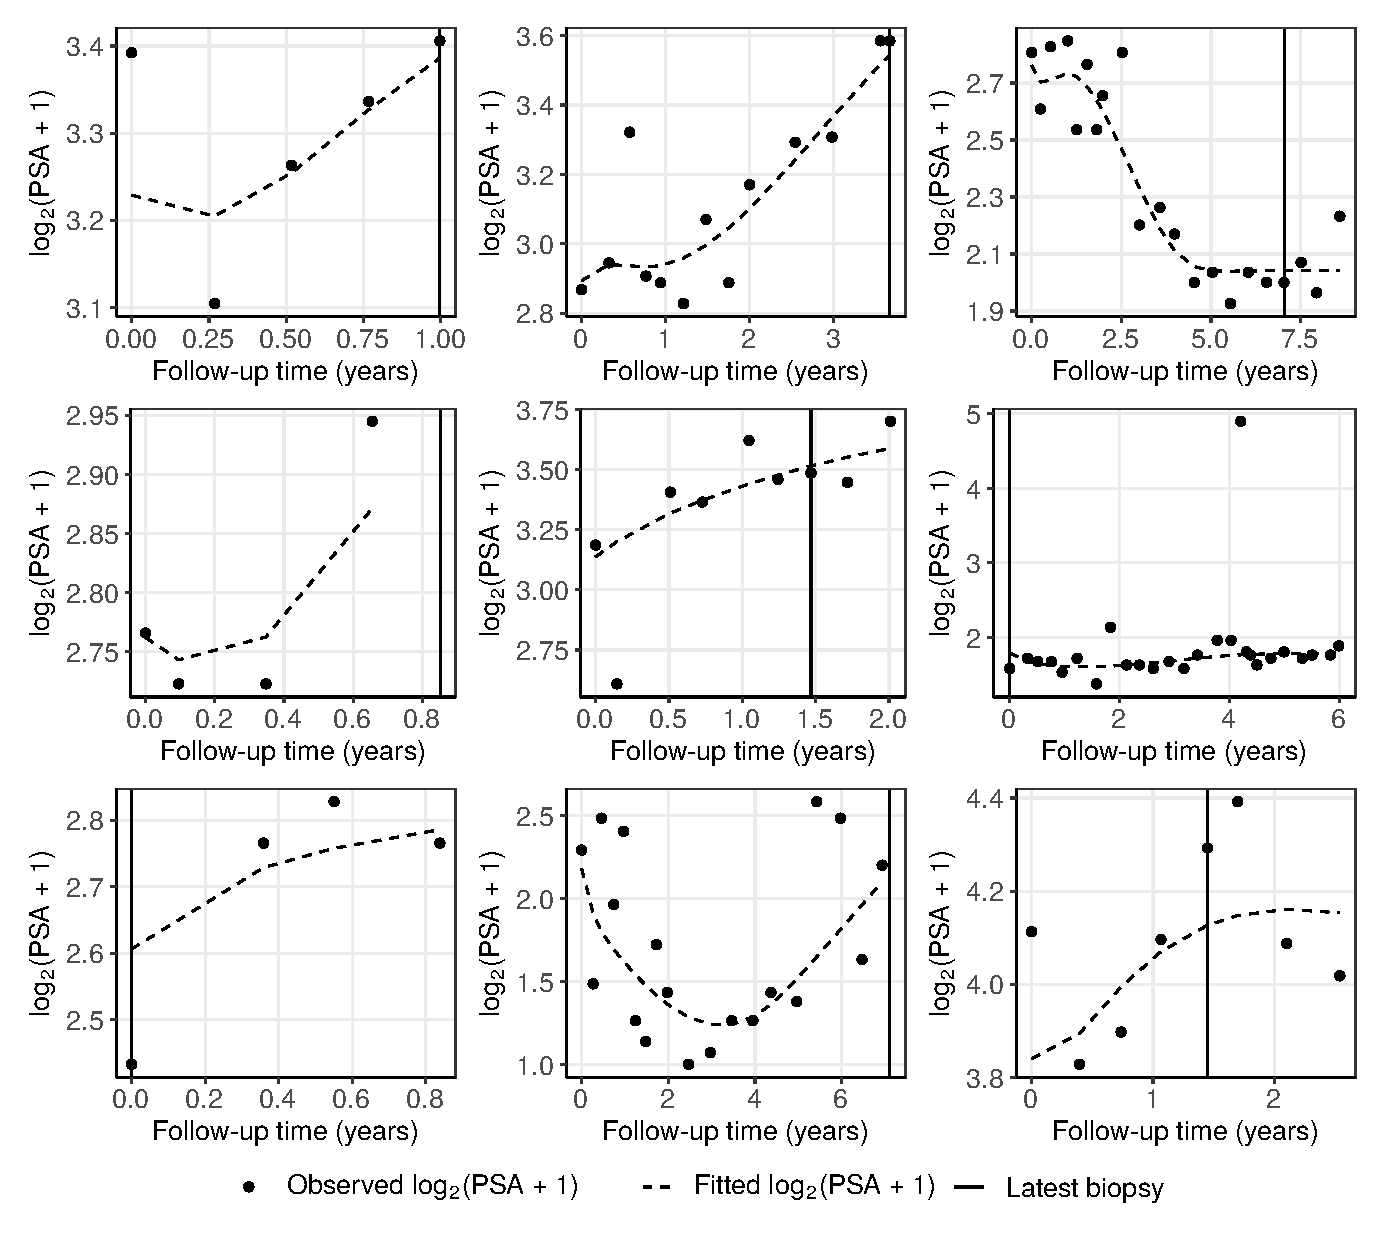
\includegraphics[width=\columnwidth]{images/fitted_9subject_psa.eps}}
\caption{Fitted versus observed ${\log_2 (\mbox{PSA} + 1)}$ profiles for nine randomly selected PRIAS patients. The fitted profiles utilize information from the observed PSA measurements, and time of the latest biopsy.}
\label{fig:fitted_9subject_psa}
\end{figure}

For the relative risk sub-model (see Equation \ref{eq:rel_risk_model}), the parameter estimates in Table~\ref{tab:PSA_survival} show that ${\log_2 (\mbox{PSA} + 1)}$ velocity and age of the patient were significantly associated with the hazard of GS7.

\begin{table}[!htb]
\small\sf\centering
\caption{Estimated mean and 95\% credible interval for the parameters of the relative risk sub-model (see Equation \ref{eq:rel_risk_model}) of the joint model fitted to the PRIAS dataset.}
\label{tab:PSA_survival}
\begin{tabular}{lrrrrr}
\hline
Variable                      & Mean   & Std. Dev & 2.5\%  & 97.5\%                 & P              \\
\hline
Age                      & 0.037    & 0.006 & 0.025  & 0.049  & \textless0.001 \\
Fitted $\log_2 (\mbox{PSA} + 1)$ value            & -0.012   & 0.076 & -0.164 & 0.135  & 0.856 \\
Fitted $\log_2 (\mbox{PSA} + 1)$ velocity             & 2.266    & 0.299 & 1.613  & 2.767  & \textless0.001   \\
\hline
\end{tabular}
\end{table}

It is important to note that since age, and ${\log_2 (\mbox{PSA} + 1)}$ value and velocity are all measured on different scales, a comparison between the corresponding parameter estimates is not easy. To this end, in Table \ref{tab:PSA_survival_easy}, we present the hazard (of GS7) ratio, for an increase in the aforementioned variables from their first to the third quartile. For example, an increase in fitted $\log_2 (\mbox{PSA} + 1)$ velocity from -0.085 to 0.308 (fitted first and third quartiles) corresponds to a hazard ratio of 2.433. The interpretation for the rest is similar.

\begin{table}[!htb]
\small\sf\centering
\caption{Hazard (of GS7) ratio and 95\% credible interval (CI), for an increase in the variables of relative risk sub-model, from their first quartile ($\mbox{Q}_1$) to their third quartile ($\mbox{Q}_3$). Except for age, quartiles for all other variables are based on their fitted values obtained from the joint model fitted to the PRIAS dataset.}
\label{tab:PSA_survival_easy}
\begin{tabular}{lrrr}
\hline
Variable                      & $\mbox{Q}_1$   & $\mbox{Q}_3$ & Hazard ratio [95\% CI] \\
\hline
Age & 61 & 71 & 1.455 [1.285, 1.631] \\
Fitted $\log_2 (\mbox{PSA} + 1)$ value & 2.360 & 3.078 & 0.991 [0.889, 1.102] \\
Fitted $\log_2 (\mbox{PSA} + 1)$ velocity & -0.085 & 0.308 & 2.433 [1.883, 2.962] \\
\hline
\end{tabular}
\end{table}

\subsection{Assumption of t-distributed (df=3) Error Terms}
\label{subsec:t-dist-assumption}
With regards to the choice of the distribution for the error term $\varepsilon$ for the PSA measurements (see Equation \ref{eq:long_model_psa}), we attempted fitting multiple joint models differing in error distribution, namely t-distribution with three, and four degrees of freedom, and a normal distribution for the error term. However, the model assumption for the error term were best met by the model with t-distribution having three degrees of freedom. The quantile-quantile plot of subject-specific residuals for the corresponding model in Panel~A of Figure~\ref{fig:qqplot}, shows that the assumption of t-distributed (df=3) errors is reasonably met by the fitted model. 

\begin{figure}[!htb]
\centerline{\includegraphics[width=\columnwidth]{images/qqplot.eps}}
\caption{Quantile-quantile plot of subject-specific residuals from the joint models fitted to the PRIAS dataset. \textbf{Panel A}: model assuming a t-distribution (df=3) for the error term $\varepsilon$ (see Equation \ref{eq:long_model_psa}). \textbf{Panel B}: model assuming a normal distribution for the error term $\varepsilon$.}
\label{fig:qqplot}
\end{figure}